\chapter{Discussion and conclusion}
\begin{figure}[htbp]
  \centering
  \begin{tabular}{ccc}
    \begin{minipage}{0.33\hsize}
      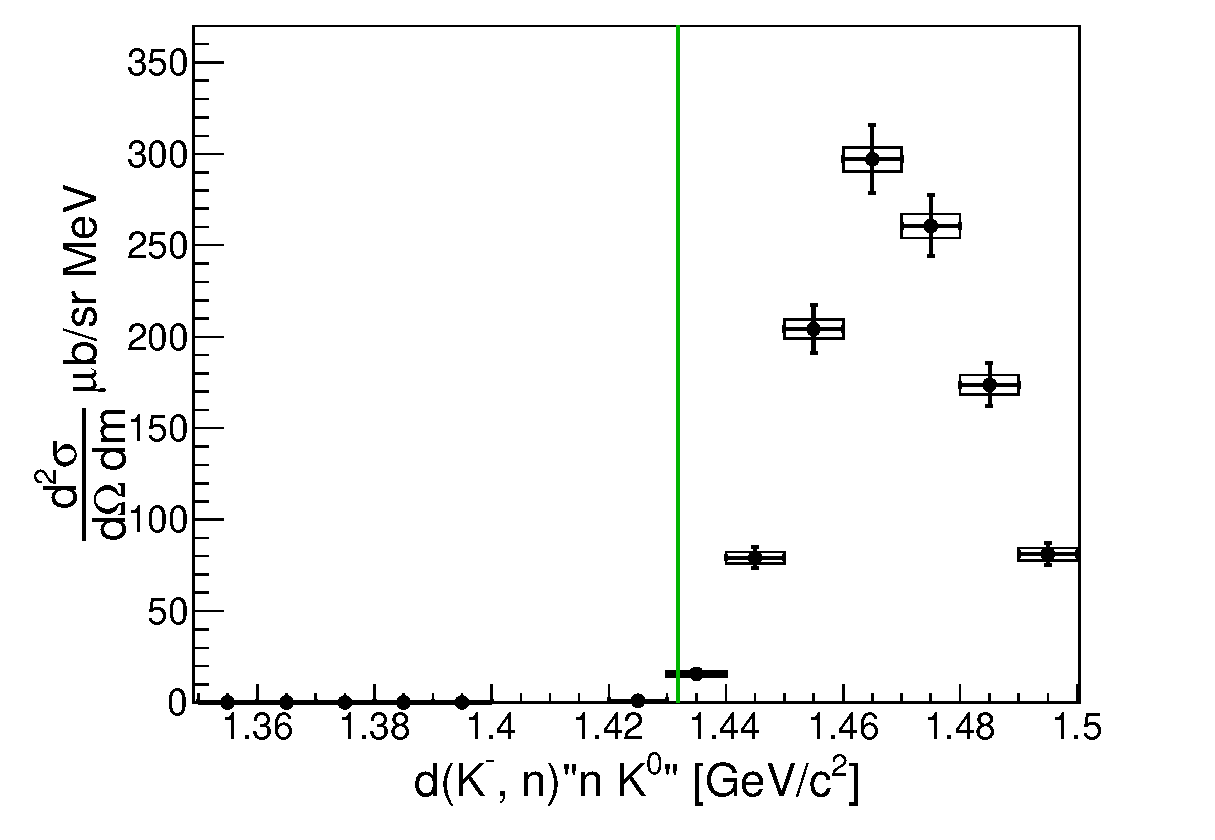
\includegraphics[width=4.5cm]{../pic/Run78/QE/K0_CS.eps}
    \end{minipage}
    \begin{minipage}{0.33\hsize}
      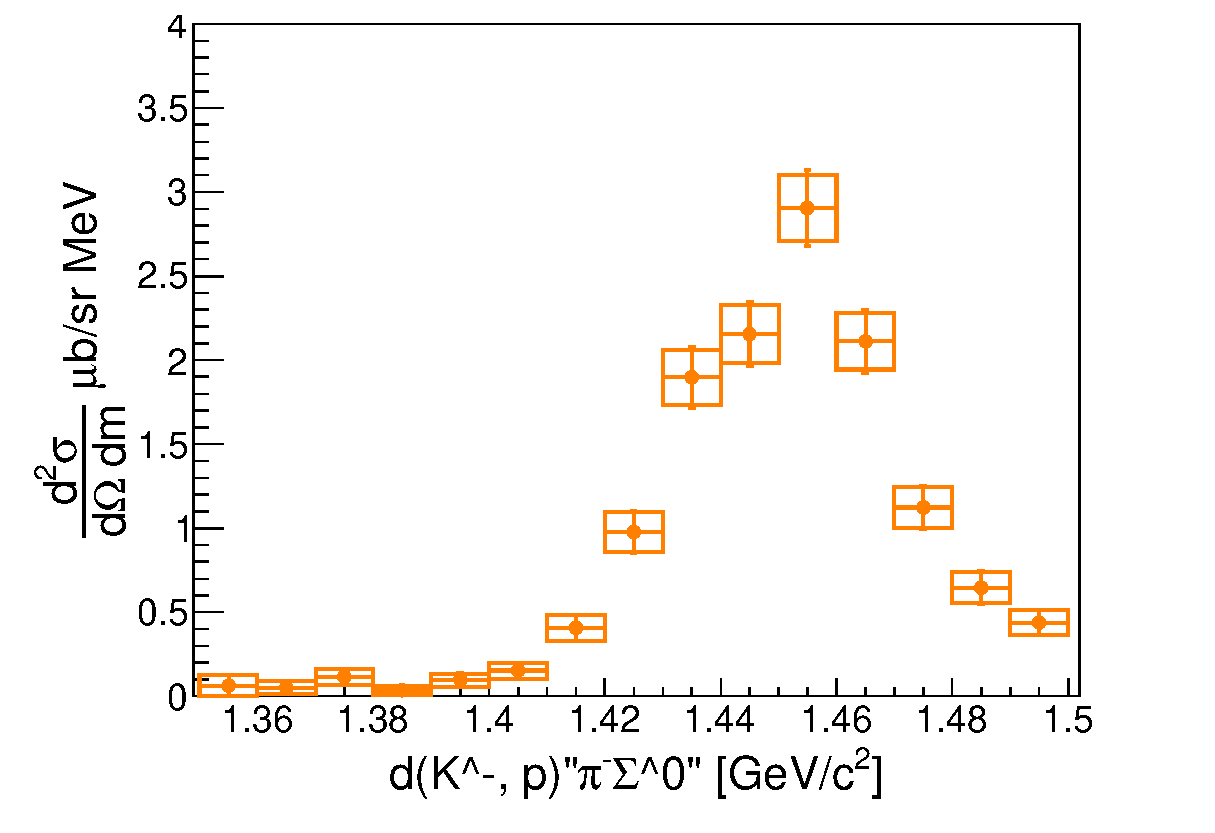
\includegraphics[width=4.5cm]{../pic/Run68/KP_ana/pimS0_CS_zoom.eps}
    \end{minipage}    
    \begin{minipage}{0.33\hsize}
      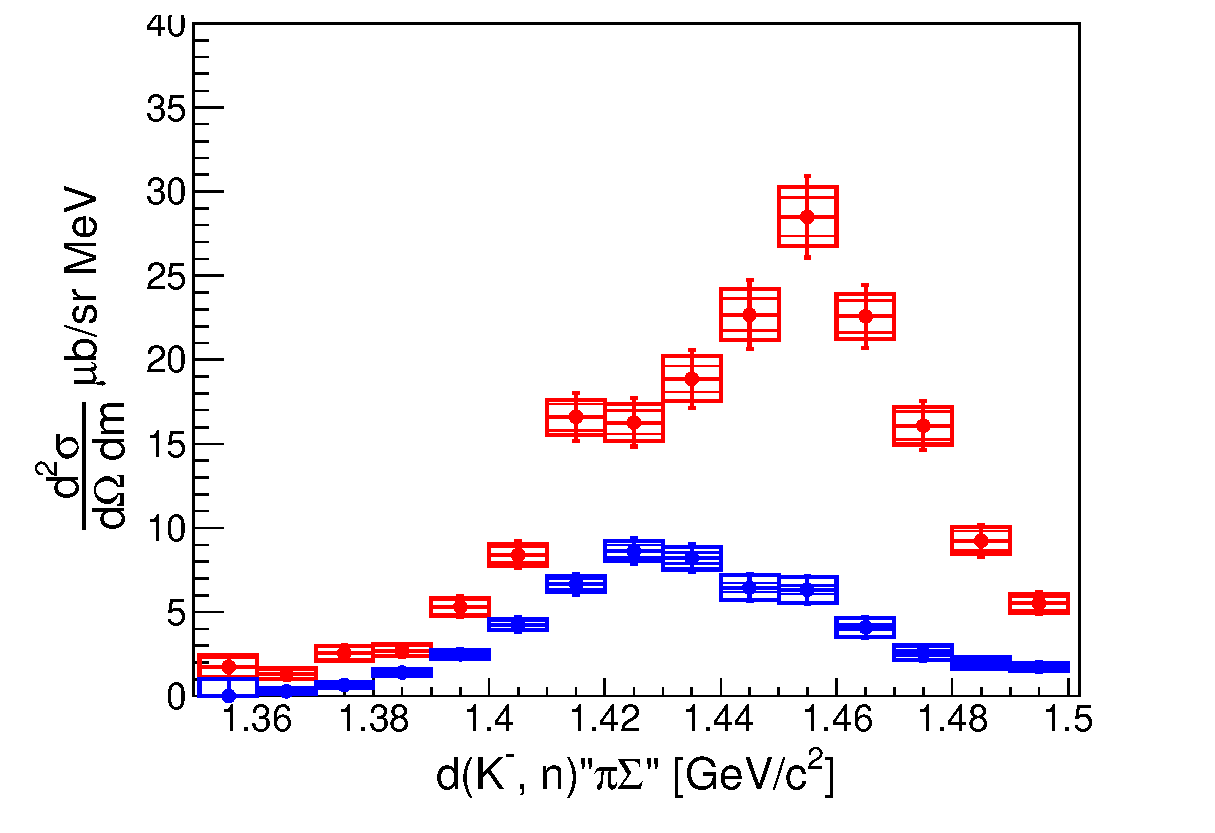
\includegraphics[width=4.5cm]{../pic/Run78/K0_ts_L1520/ChargeCS_after.eps}
    \end{minipage}
  \end{tabular}
  \caption{
    Obtained cross sections. Left, center and right figures shows $d(K^-, n)"n K^0"$, $d(K^-, p)"\pi^-\Sigma^0"$ and $d(K^-, n)"\pi^{\mp}\Sigma^{\pm}"$, respectively.
    Boxes indicate independent errors for each bins. In left and center figure, boxes is only staticial error of events.
    Only right figure, there are fitting error to separate $\pi^-\Sigma^+$ and $\pi^+\Sigma^-$ modes which indicates outer boxes as convolved error by RMS with statical errors.
    Error bars indicate conversion factor to cross sections convolved error by RMS.
  }
  \label{fig:obtainedCS}
\end{figure}
We obatain $d(K^-, N)$ spactra identified four type final state (Fig\ref{fig:obtainedCS}) to search the $\bar{K}N$ scattering amplitude near the $\bar{K}N$ threshold that includes below the threshold.
First one is the $d(K^-, n)"n K^0"$ spectrum by which can not measured below the threshold, but it is good prove to measure 1-step, so called quasi-elastic reaction.
Because fermi momentum in the deuteron was samll ($<0.1 GeV/c$), $d(K^, n)$ spectrum should be araised from the $\bar{K}N$ threshold and make bump structure just above the threshold.
Actually, obatained spatrum made a bump structure around $1.45GeV/c^{2}$ which cresspond to fermi motion effect.
In appendix.X, we discussed more detail of $nK^0$ final state.

Also, we have measured the three type $\pi\Sigma$ final state that can be measured below the $\bar{K}N$ threshold.
These reactions are conceivable that 2-step reaction in which $K^-$ kicks a nucleon out and the recoiled $\bar{K}$ reacts with residual nucleon and becoume $\pi\Sigma$.
We measured $d(K^-, p)"\pi^-\Sigma^0"$ final state which is pure $I=1$ scattering amplitude that is expected to supressed around the $\bar{K}N$ threshold due to no pole.
Obtained spectrum was strongly suppressed below the $\bar{K}N$ threshold and similar structure to quasi-elastic was observed aboved the threshold.
We also measured $d(K^-, n)\pi^{\mp}\Sigma^{\pm}$ spectra which include $I=0$ and $I=1$ scattering amplitude.

The interferance term appears the difference of two spectra which was observed, espacially above the threshold.
The interferance term can be canceled by average operation.

\begin{figure}
  \centering
  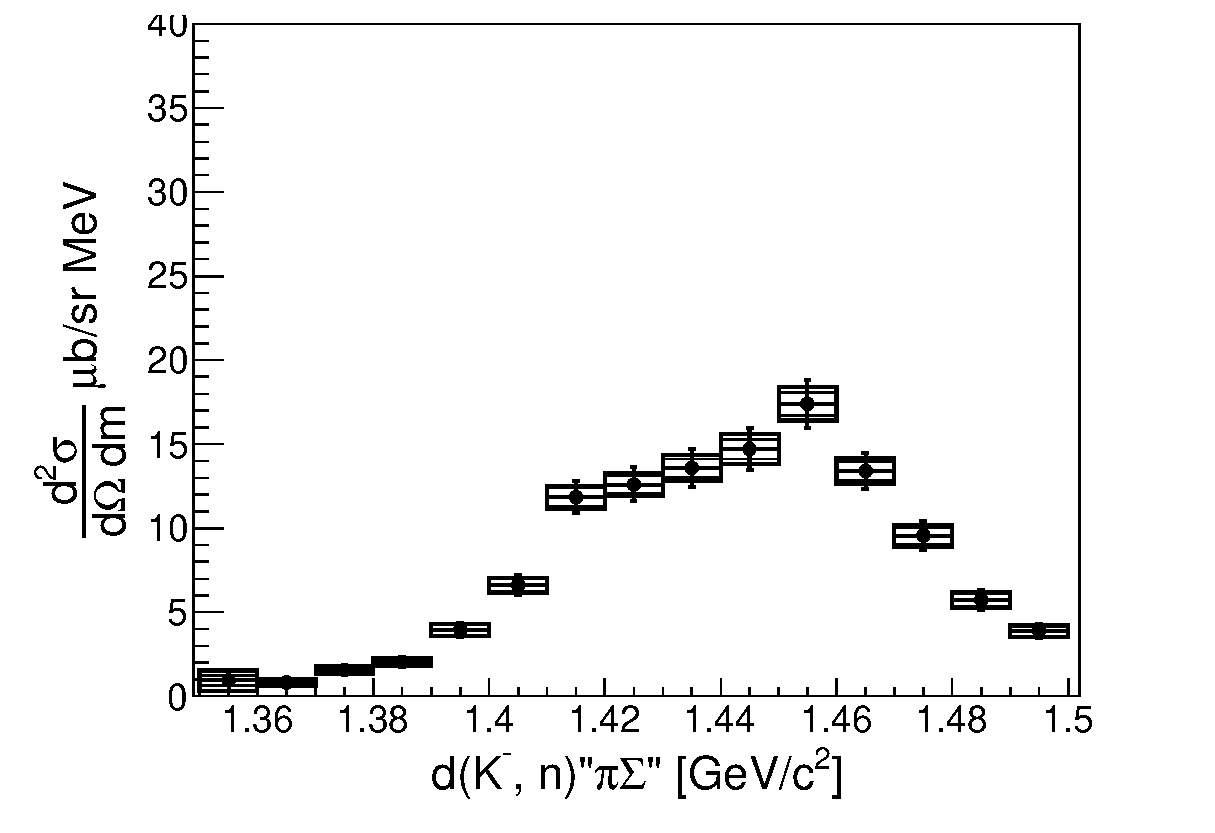
\includegraphics[width=12cm]{../pic/Run78/K0_ts_L1520/ChargeCS_ave_after.eps}
  \caption{
    Average spectrum of the $d(K^-, n)"\pi^{\mp}\Sigma^{\pm}"$ that is canceled the interferance term.
    Errors indicated as Fig.\ref{fig:obtainedCS}.
  }
  \label{fig:ChargeCS}
\end{figure}
